\documentclass{jpconf}
\usepackage[utf8]{inputenc}
\usepackage{fontspec}
\usepackage{DFormat}
\usepackage{amsmath}
\usepackage{amsthm}
\usepackage{amssymb}
\usepackage{hyperref}
\hypersetup{%
	pdfborder=false,%
	linkcolor=teal%
}%

\usepackage{listings}
\usepackage{xcolor}

\usepackage{pgfplots}
%\usepgfplotslibrary{groupplots}

%\usepackage{apacite}
\usepackage{epstopdf}
\usepackage{graphicx}

\usepackage{caption}
\usepackage{subcaption}
\usepackage{pstricks}
\usepackage{pgf}
\usepackage{tikz}

%Let us cee if it works

\definecolor{mygreen}{rgb}{0,0.6,0}
\definecolor{mygray}{rgb}{1.0,0.5,0.5}
\definecolor{mymauve}{rgb}{0.58,0,0.82}
\lstset{ %
backgroundcolor=\color{white}, % choose the background color; you must add \usepackage{color} or \usepackage{xcolor}
basicstyle=\footnotesize \ttfamily, % the size of the fonts that are used for the code
breakatwhitespace=false, % sets if automatic breaks should only happen at whitespace
breaklines=true, % sets automatic line breaking 
%captionpos=b, % sets the caption-position to bottom
commentstyle=\color{mygreen}, % comment style
deletekeywords={...}, % if you want to delete keywords from the given language
escapeinside={\%*}{*)}, % if you want to add LaTeX within your code
extendedchars=true, % lets you use non-ASCII characters; for 8-bits encodings only, does not work with UTF-8
%frame=single, % adds a frame around the code 
keywordstyle=\color{blue}, % keyword style 
morekeywords={cin,cout}, % if you want to add more keywordsto the set
identifierstyle=,
numbers=none, % where to put the linumbers; possible values are (none, left, right)
numbersep=5pt, % how far the line-numbers are from the code
numberstyle=\tiny\color{mygray}, % the style that is used for theline-numbers
rulecolor=\color{black}, % if not set, the frame-color may be changed on line-breaks within not-black text (e.g. comments (green here))
showspaces=false, % show spaces everywhere adding particular underscores; it overrides ‚showstringspaces‚
showstringspaces=false, % underline spaces within strings only
showtabs=false, % show tabs within strings adding particular underscores
stepnumber=1, % the step between two line-numbers. If it‚s 1, each line will be numbered
stringstyle=\color{mymauve}, % string literal style
tabsize=2, % sets default tabsize to 2 spaces
%title=\lstname % show the filename of files included with \lstinputlisting; also try caption instead of title
%directives={include,define}
}

%Let Us really see upto this

\lstset{float,frame=rectangle}

\usetikzlibrary{calendar,arrows,folding}

\bibliographystyle{plain}


%\stAuthorName{Madhave Humagain$^{1\#}$, ~ Prakash Gautam$^{2\#}$}
%\stAuthorEmail{$^1$scimad2.71@gmail.com ~ $^2$pranphy@gmail.com}
%\stOrganization{$^{\#}$The Delta Finders}

\theoremstyle{definition} \newtheorem{Definition}{Def{\,}inition} 

\begin{document}
	\stTitle{A simple geometrical series that converges to $\pi$}
	\stConfTitle 
\begin{abstract}
This paper describes one of many possible ways to calculate the value of $\pi$ with a geometrical series. This method will be particulary useful to calculate the value of $\pi$ with iterative approach taking terms as per the required precision.
\end{abstract}


\section{Introduction}
$\pi$ comes flying all over high school mathematics. Beginner studensts often confuse the number $\pi$ with $180^0$ or $\frac{22}{7}$ which in fact is just a crude approximation of $\pi$. The approach taken in this paper will help beginners understand what actually is $\pi$.


\section{Historical Note}
Intuitively we can also guess that if we make bigger and bigger circle both diameter and circumference increase. It makes us wonder if there is a certain relation between the diameter and circumference of circle. Curious Babylonians in the early ages, out of similar curiosity, tried to measure the ratio of circumference to diameter. Unsurprisingly they found the ratio was close to $3$. For various observations they found this ratio was always closer to 3, little greater than 3 and never larger than 4. They didn't precisely know the value of the ratio. So they named the ratio a magical symbol, which is $\pi$.
\section{Random }
Some random sentences to begin the section formally.
\begin{Definition}
	\emph{ $\pi$ is the ratio of circumference to diameter of a circle. i.e., $\pi = \frac{C}{d}$, where $C$ is the circumference, $d$ is the diameter of circle}
\end{Definition}
Using this definition of circumference of circle, it is not hard to work out the area of circle. As it turns out the area of circle in terms of the named constant comes out to be \footnote{The derivation of $A = \pi r^2$ is given in Appendix A}\[ A = \pi r^2 \]
So far we don't know what is the value of number denoted by $\pi$. If we take a circle of unit radius, i.e., $r = 1$ then the area of circle turns, numerically, out to be $\pi$. We now calculate the area of unit circle geometrically. The area we calculate will, numerically, be the value of $\pi$ which we all are looking for in this paper.
			
\section{Area of unit circle}


\begin{figure}
	\centering
	\begin{subfigure}[b]{0.30\textwidth}
		\centering
		\scalebox{0.8}{%LaTeX with PSTricks extensions
%%Creator: inkscape 0.91
%%Please note this file requires PSTricks extensions
\psset{xunit=.5pt,yunit=.5pt,runit=.5pt}
\begin{pspicture}(337.03078323,338.58233174)
{
\newrgbcolor{curcolor}{0 0 0}
\pscustom[linewidth=2,linecolor=curcolor]
{
\newpath
\moveto(321.00000027,161.00000761)
\curveto(321.00000027,72.63444767)(249.36556021,1.00000761)(161.00000027,1.00000761)
\curveto(72.63444033,1.00000761)(1.00000027,72.63444767)(1.00000027,161.00000761)
\curveto(1.00000027,249.36556755)(72.63444033,321.00000761)(161.00000027,321.00000761)
\curveto(249.36556021,321.00000761)(321.00000027,249.36556755)(321.00000027,161.00000761)
\closepath
}
}
{
\newrgbcolor{curcolor}{0 0 0}
\pscustom[linewidth=2,linecolor=curcolor]
{
\newpath
\moveto(161.00002,321.00004174)
\lineto(161.00002,161.00004174)
\lineto(321.00002,161.00004174)
\lineto(321.00002,161.00004174)
}
}
{
\newrgbcolor{curcolor}{0 0 0}
\pscustom[linewidth=2,linecolor=curcolor]
{
\newpath
\moveto(161.00002,321.00004174)
\lineto(321.00002,161.00004174)
\lineto(321.00002,161.00004174)
}
}
{
\newrgbcolor{curcolor}{0 0 0}
\pscustom[linestyle=none,fillstyle=solid,fillcolor=curcolor]
{
\newpath
\moveto(161.74673895,338.24022984)
\lineto(161.73929588,338.26075574)
\lineto(161.73185282,338.28128164)
\lineto(161.72440975,338.29838656)
\lineto(161.71696669,338.31891247)
\lineto(161.70952362,338.33601739)
\lineto(161.70208056,338.3531223)
\lineto(161.69091596,338.37022722)
\lineto(161.6834729,338.38733214)
\lineto(161.67602983,338.40101608)
\lineto(161.66858677,338.418121)
\lineto(161.6611437,338.43180493)
\lineto(161.6499791,338.44548887)
\lineto(161.64253604,338.45917281)
\lineto(161.63137144,338.46943576)
\lineto(161.62392838,338.48311969)
\lineto(161.61276378,338.49338264)
\lineto(161.60159918,338.5036456)
\lineto(161.59043458,338.51390855)
\lineto(161.57554845,338.5241715)
\lineto(161.56438386,338.53101347)
\lineto(161.54949773,338.54127642)
\lineto(161.5346116,338.54811839)
\lineto(161.51972547,338.55496035)
\lineto(161.5011178,338.55838134)
\lineto(161.48251014,338.56522331)
\lineto(161.46390248,338.56864429)
\lineto(161.44529482,338.57206527)
\lineto(161.42296562,338.57548626)
\lineto(161.40063643,338.57890724)
\lineto(161.3745857,338.57890724)
\lineto(161.34853497,338.58232823)
\lineto(161.33737038,338.58232823)
\lineto(161.32248425,338.58232823)
\curveto(161.02476165,338.58232823)(160.96893866,338.47969871)(160.87590035,338.24022984)
\lineto(157.03900037,328.04911882)
\curveto(156.70778398,327.18018891)(155.96719902,326.92361512)(154.96238525,326.9065102)
\lineto(154.96238525,326.37967868)
\lineto(158.98536185,326.37967868)
\lineto(158.98536185,326.9065102)
\curveto(158.05870027,326.9065102)(157.59723024,327.33413319)(157.59723024,327.77886109)
\curveto(157.59723024,327.82675487)(157.6158379,327.99780406)(157.63444557,328.0320139)
\lineto(158.4866765,330.26591638)
\lineto(158.69136079,330.7927479)
\lineto(160.76425438,336.33132082)
\lineto(162.85947716,330.7927479)
\lineto(158.69136079,330.7927479)
\lineto(158.4866765,330.26591638)
\lineto(163.06416144,330.26591638)
\lineto(164.04664602,327.65570567)
\curveto(164.06525368,327.59070698)(164.102469,327.48807746)(164.102469,327.41965778)
\curveto(164.102469,326.9065102)(163.06416144,326.9065102)(162.56547609,326.9065102)
\lineto(162.56547609,326.37967868)
\lineto(167.66025405,326.37967868)
\lineto(167.66025405,326.9065102)
\lineto(167.32903766,326.9065102)
\curveto(166.21629945,326.9065102)(165.95579217,327.02624464)(165.75482942,327.59070698)
\closepath
}
}
{
\newrgbcolor{curcolor}{0 0 0}
\pscustom[linewidth=0,linecolor=curcolor]
{
\newpath
\moveto(161.74673895,338.24022984)
\lineto(161.73929588,338.26075574)
\lineto(161.73185282,338.28128164)
\lineto(161.72440975,338.29838656)
\lineto(161.71696669,338.31891247)
\lineto(161.70952362,338.33601739)
\lineto(161.70208056,338.3531223)
\lineto(161.69091596,338.37022722)
\lineto(161.6834729,338.38733214)
\lineto(161.67602983,338.40101608)
\lineto(161.66858677,338.418121)
\lineto(161.6611437,338.43180493)
\lineto(161.6499791,338.44548887)
\lineto(161.64253604,338.45917281)
\lineto(161.63137144,338.46943576)
\lineto(161.62392838,338.48311969)
\lineto(161.61276378,338.49338264)
\lineto(161.60159918,338.5036456)
\lineto(161.59043458,338.51390855)
\lineto(161.57554845,338.5241715)
\lineto(161.56438386,338.53101347)
\lineto(161.54949773,338.54127642)
\lineto(161.5346116,338.54811839)
\lineto(161.51972547,338.55496035)
\lineto(161.5011178,338.55838134)
\lineto(161.48251014,338.56522331)
\lineto(161.46390248,338.56864429)
\lineto(161.44529482,338.57206527)
\lineto(161.42296562,338.57548626)
\lineto(161.40063643,338.57890724)
\lineto(161.3745857,338.57890724)
\lineto(161.34853497,338.58232823)
\lineto(161.33737038,338.58232823)
\lineto(161.32248425,338.58232823)
\curveto(161.02476165,338.58232823)(160.96893866,338.47969871)(160.87590035,338.24022984)
\lineto(157.03900037,328.04911882)
\curveto(156.70778398,327.18018891)(155.96719902,326.92361512)(154.96238525,326.9065102)
\lineto(154.96238525,326.37967868)
\lineto(158.98536185,326.37967868)
\lineto(158.98536185,326.9065102)
\curveto(158.05870027,326.9065102)(157.59723024,327.33413319)(157.59723024,327.77886109)
\curveto(157.59723024,327.82675487)(157.6158379,327.99780406)(157.63444557,328.0320139)
\lineto(158.4866765,330.26591638)
\lineto(158.69136079,330.7927479)
\lineto(160.76425438,336.33132082)
\lineto(162.85947716,330.7927479)
\lineto(158.69136079,330.7927479)
\lineto(158.4866765,330.26591638)
\lineto(163.06416144,330.26591638)
\lineto(164.04664602,327.65570567)
\curveto(164.06525368,327.59070698)(164.102469,327.48807746)(164.102469,327.41965778)
\curveto(164.102469,326.9065102)(163.06416144,326.9065102)(162.56547609,326.9065102)
\lineto(162.56547609,326.37967868)
\lineto(167.66025405,326.37967868)
\lineto(167.66025405,326.9065102)
\lineto(167.32903766,326.9065102)
\curveto(166.21629945,326.9065102)(165.95579217,327.02624464)(165.75482942,327.59070698)
\closepath
}
}
{
\newrgbcolor{curcolor}{0 0 0}
\pscustom[linestyle=none,fillstyle=solid,fillcolor=curcolor]
{
\newpath
\moveto(333.53269308,160.78854782)
\lineto(333.69632497,160.81807956)
\lineto(333.85632059,160.85417391)
\lineto(334.01267996,160.89354957)
\lineto(334.16903932,160.93620652)
\lineto(334.31812615,160.98542609)
\lineto(334.46357672,161.03464566)
\lineto(334.60539103,161.09042784)
\lineto(334.74356907,161.14949132)
\lineto(334.87811085,161.21183611)
\lineto(335.00901636,161.2741809)
\lineto(335.13628561,161.3430883)
\lineto(335.25628233,161.415277)
\lineto(335.37264278,161.490747)
\lineto(335.48536697,161.56949831)
\lineto(335.5944549,161.64824962)
\lineto(335.6962703,161.73356354)
\lineto(335.79444943,161.81887746)
\lineto(335.88535604,161.90747269)
\lineto(335.97262638,161.99934922)
\lineto(336.0526242,162.09122575)
\lineto(336.12898574,162.18638358)
\lineto(336.19807476,162.28482272)
\lineto(336.25989126,162.38326186)
\lineto(336.31807148,162.4849823)
\lineto(336.36897918,162.58998405)
\lineto(336.41261436,162.69498579)
\lineto(336.45261326,162.79998754)
\lineto(336.48170338,162.90827059)
\lineto(336.50715723,163.01655364)
\lineto(336.52533855,163.128118)
\lineto(336.53624734,163.23968236)
\lineto(336.5398836,163.35452802)
\curveto(336.5398836,164.77533291)(334.87447458,166.11410519)(332.51817535,166.11410519)
\lineto(332.39454237,165.60878428)
\curveto(334.150858,165.60878428)(334.78356797,164.21751113)(334.78356797,163.35452802)
\curveto(334.78356797,162.30451055)(333.8963195,160.93292522)(331.88546537,160.93292522)
\lineto(329.26008259,160.93292522)
\lineto(329.26008259,160.57526302)
\lineto(332.66362592,160.57526302)
\curveto(334.45994046,160.57526302)(335.21991968,159.05273768)(335.21991968,157.95678194)
\curveto(335.21991968,156.79848142)(334.27812725,155.45642783)(332.41272369,155.45642783)
\lineto(332.41272369,155.45642783)
\lineto(330.14733107,155.45642783)
\curveto(329.29644523,155.45642783)(329.26008259,155.5712735)(329.26008259,156.11268876)
\lineto(329.26008259,160.57526302)
\lineto(329.26008259,160.93292522)
\lineto(329.26008259,164.95252336)
\curveto(329.26008259,165.49393862)(329.29644523,165.60878428)(330.14733107,165.60878428)
\lineto(332.39454237,165.60878428)
\lineto(332.51817535,166.11410519)
\lineto(325.88926564,166.11410519)
\lineto(325.88926564,165.60878428)
\lineto(326.32561735,165.60878428)
\curveto(327.71830655,165.60878428)(327.75830546,165.42831253)(327.75830546,164.840959)
\lineto(327.75830546,156.22753442)
\curveto(327.75830546,155.63689959)(327.71830655,155.45642783)(326.32561735,155.45642783)
\lineto(325.88926564,155.45642783)
\lineto(325.88926564,154.95110693)
\lineto(332.9908897,154.95110693)
\curveto(335.4017329,154.95110693)(337.03077928,156.40472487)(337.03077928,157.94365673)
\curveto(337.03077928,159.36446162)(335.5435472,160.58838824)(333.53269308,160.78854782)
\closepath
}
}
{
\newrgbcolor{curcolor}{0 0 0}
\pscustom[linewidth=0,linecolor=curcolor]
{
\newpath
\moveto(333.53269308,160.78854782)
\lineto(333.69632497,160.81807956)
\lineto(333.85632059,160.85417391)
\lineto(334.01267996,160.89354957)
\lineto(334.16903932,160.93620652)
\lineto(334.31812615,160.98542609)
\lineto(334.46357672,161.03464566)
\lineto(334.60539103,161.09042784)
\lineto(334.74356907,161.14949132)
\lineto(334.87811085,161.21183611)
\lineto(335.00901636,161.2741809)
\lineto(335.13628561,161.3430883)
\lineto(335.25628233,161.415277)
\lineto(335.37264278,161.490747)
\lineto(335.48536697,161.56949831)
\lineto(335.5944549,161.64824962)
\lineto(335.6962703,161.73356354)
\lineto(335.79444943,161.81887746)
\lineto(335.88535604,161.90747269)
\lineto(335.97262638,161.99934922)
\lineto(336.0526242,162.09122575)
\lineto(336.12898574,162.18638358)
\lineto(336.19807476,162.28482272)
\lineto(336.25989126,162.38326186)
\lineto(336.31807148,162.4849823)
\lineto(336.36897918,162.58998405)
\lineto(336.41261436,162.69498579)
\lineto(336.45261326,162.79998754)
\lineto(336.48170338,162.90827059)
\lineto(336.50715723,163.01655364)
\lineto(336.52533855,163.128118)
\lineto(336.53624734,163.23968236)
\lineto(336.5398836,163.35452802)
\curveto(336.5398836,164.77533291)(334.87447458,166.11410519)(332.51817535,166.11410519)
\lineto(332.39454237,165.60878428)
\curveto(334.150858,165.60878428)(334.78356797,164.21751113)(334.78356797,163.35452802)
\curveto(334.78356797,162.30451055)(333.8963195,160.93292522)(331.88546537,160.93292522)
\lineto(329.26008259,160.93292522)
\lineto(329.26008259,160.57526302)
\lineto(332.66362592,160.57526302)
\curveto(334.45994046,160.57526302)(335.21991968,159.05273768)(335.21991968,157.95678194)
\curveto(335.21991968,156.79848142)(334.27812725,155.45642783)(332.41272369,155.45642783)
\lineto(332.41272369,155.45642783)
\lineto(330.14733107,155.45642783)
\curveto(329.29644523,155.45642783)(329.26008259,155.5712735)(329.26008259,156.11268876)
\lineto(329.26008259,160.57526302)
\lineto(329.26008259,160.93292522)
\lineto(329.26008259,164.95252336)
\curveto(329.26008259,165.49393862)(329.29644523,165.60878428)(330.14733107,165.60878428)
\lineto(332.39454237,165.60878428)
\lineto(332.51817535,166.11410519)
\lineto(325.88926564,166.11410519)
\lineto(325.88926564,165.60878428)
\lineto(326.32561735,165.60878428)
\curveto(327.71830655,165.60878428)(327.75830546,165.42831253)(327.75830546,164.840959)
\lineto(327.75830546,156.22753442)
\curveto(327.75830546,155.63689959)(327.71830655,155.45642783)(326.32561735,155.45642783)
\lineto(325.88926564,155.45642783)
\lineto(325.88926564,154.95110693)
\lineto(332.9908897,154.95110693)
\curveto(335.4017329,154.95110693)(337.03077928,156.40472487)(337.03077928,157.94365673)
\curveto(337.03077928,159.36446162)(335.5435472,160.58838824)(333.53269308,160.78854782)
\closepath
}
}
{
\newrgbcolor{curcolor}{0.54901962 0.52156864 0.52156864}
\pscustom[linestyle=none,fillstyle=solid,fillcolor=curcolor]
{
\newpath
\moveto(162.47891,239.88549174)
\lineto(162.47891,317.56283174)
\lineto(239.97891,240.06530174)
\curveto(282.60391,197.44165174)(317.47891,162.48685174)(317.47891,162.38796174)
\curveto(317.47891,162.28906174)(282.60391,162.20815174)(239.97891,162.20815174)
\lineto(162.47891,162.20815174)
\lineto(162.47891,239.88549174)
\closepath
}
}
{
\newrgbcolor{curcolor}{0 0 0}
\pscustom[linestyle=none,fillstyle=solid,fillcolor=curcolor]
{
\newpath
\moveto(158.24171634,158.12883645)
\lineto(158.23553754,158.45165812)
\lineto(158.21700116,158.7744798)
\lineto(158.18301778,159.08699865)
\lineto(158.1366768,159.3995175)
\lineto(158.08106764,159.70173354)
\lineto(158.01001148,160.0005153)
\lineto(157.92968713,160.29242851)
\lineto(157.83700519,160.57747318)
\lineto(157.73196565,160.8556493)
\lineto(157.61765792,161.12695688)
\lineto(157.49408199,161.38796164)
\lineto(157.36123787,161.64209785)
\lineto(157.21603616,161.88593124)
\lineto(157.06465565,162.12289608)
\lineto(156.90091755,162.34955811)
\lineto(156.73100065,162.56591731)
\lineto(156.55181556,162.7719737)
\lineto(156.36645168,162.96772727)
\lineto(156.17181959,163.15317802)
\lineto(155.97100871,163.32832595)
\lineto(155.76401904,163.48973678)
\lineto(155.54776117,163.6408448)
\lineto(155.3284139,163.77478145)
\lineto(155.09979844,163.90184956)
\lineto(154.86809358,164.0117463)
\lineto(154.63329932,164.11134022)
\lineto(154.38923687,164.19376277)
\lineto(154.14208502,164.26244823)
\lineto(153.89184377,164.3173966)
\lineto(153.63851313,164.35517361)
\lineto(153.37900368,164.37921352)
\lineto(153.11949424,164.38951634)
\lineto(153.11949424,163.9602322)
\curveto(154.45720363,163.9602322)(156.6599445,162.74793379)(156.6599445,158.36923557)
\curveto(156.6599445,153.83256078)(154.54988557,152.39703462)(153.13494123,152.39703462)
\lineto(153.13494123,152.39703462)
\curveto(151.65511952,152.39703462)(149.59449097,153.90124624)(149.59449097,158.36923557)
\curveto(149.59449097,162.79601361)(151.84048341,163.9602322)(153.11949424,163.9602322)
\lineto(153.11949424,164.38951634)
\curveto(150.36375111,164.38951634)(148.00962973,161.65240067)(148.00962973,158.12883645)
\curveto(148.00962973,154.6224436)(150.3791981,151.95057912)(153.11949424,151.95057912)
\curveto(155.91848895,151.95057912)(158.24171634,154.67052342)(158.24171634,158.12883645)
\closepath
}
}
{
\newrgbcolor{curcolor}{0 0 0}
\pscustom[linewidth=0,linecolor=curcolor]
{
\newpath
\moveto(158.24171634,158.12883645)
\lineto(158.23553754,158.45165812)
\lineto(158.21700116,158.7744798)
\lineto(158.18301778,159.08699865)
\lineto(158.1366768,159.3995175)
\lineto(158.08106764,159.70173354)
\lineto(158.01001148,160.0005153)
\lineto(157.92968713,160.29242851)
\lineto(157.83700519,160.57747318)
\lineto(157.73196565,160.8556493)
\lineto(157.61765792,161.12695688)
\lineto(157.49408199,161.38796164)
\lineto(157.36123787,161.64209785)
\lineto(157.21603616,161.88593124)
\lineto(157.06465565,162.12289608)
\lineto(156.90091755,162.34955811)
\lineto(156.73100065,162.56591731)
\lineto(156.55181556,162.7719737)
\lineto(156.36645168,162.96772727)
\lineto(156.17181959,163.15317802)
\lineto(155.97100871,163.32832595)
\lineto(155.76401904,163.48973678)
\lineto(155.54776117,163.6408448)
\lineto(155.3284139,163.77478145)
\lineto(155.09979844,163.90184956)
\lineto(154.86809358,164.0117463)
\lineto(154.63329932,164.11134022)
\lineto(154.38923687,164.19376277)
\lineto(154.14208502,164.26244823)
\lineto(153.89184377,164.3173966)
\lineto(153.63851313,164.35517361)
\lineto(153.37900368,164.37921352)
\lineto(153.11949424,164.38951634)
\lineto(153.11949424,163.9602322)
\curveto(154.45720363,163.9602322)(156.6599445,162.74793379)(156.6599445,158.36923557)
\curveto(156.6599445,153.83256078)(154.54988557,152.39703462)(153.13494123,152.39703462)
\lineto(153.13494123,152.39703462)
\curveto(151.65511952,152.39703462)(149.59449097,153.90124624)(149.59449097,158.36923557)
\curveto(149.59449097,162.79601361)(151.84048341,163.9602322)(153.11949424,163.9602322)
\lineto(153.11949424,164.38951634)
\curveto(150.36375111,164.38951634)(148.00962973,161.65240067)(148.00962973,158.12883645)
\curveto(148.00962973,154.6224436)(150.3791981,151.95057912)(153.11949424,151.95057912)
\curveto(155.91848895,151.95057912)(158.24171634,154.67052342)(158.24171634,158.12883645)
\closepath
}
}
\end{pspicture}
}
		\caption{Area of first triangle}
		\label{fig:a_0}
	\end{subfigure}%
	\begin{subfigure}[b]{0.30\textwidth}
		\centering
		\scalebox{0.8}{%LaTeX with PSTricks extensions
%%Creator: inkscape 0.91
%%Please note this file requires PSTricks extensions
\psset{xunit=.5pt,yunit=.5pt,runit=.5pt}
\begin{pspicture}(337.03075619,338.58230471)
{
\newrgbcolor{curcolor}{0 0 0}
\pscustom[linewidth=2,linecolor=curcolor]
{
\newpath
\moveto(321,161.00000157)
\curveto(321,72.63444163)(249.36555994,1.00000157)(161,1.00000157)
\curveto(72.63444006,1.00000157)(1,72.63444163)(1,161.00000157)
\curveto(1,249.36556151)(72.63444006,321.00000157)(161,321.00000157)
\curveto(249.36555994,321.00000157)(321,249.36556151)(321,161.00000157)
\closepath
}
}
{
\newrgbcolor{curcolor}{0 0 0}
\pscustom[linewidth=2,linecolor=curcolor]
{
\newpath
\moveto(161,321.00001471)
\lineto(161,161.00001471)
\lineto(321,161.00001471)
\lineto(321,161.00001471)
}
}
{
\newrgbcolor{curcolor}{0 0 0}
\pscustom[linewidth=2,linecolor=curcolor]
{
\newpath
\moveto(161,321.00001471)
\lineto(321,161.00001471)
\lineto(321,161.00001471)
}
}
{
\newrgbcolor{curcolor}{0 0 0}
\pscustom[linewidth=2,linecolor=curcolor]
{
\newpath
\moveto(161,161.00001471)
\lineto(274,274.00001471)
}
}
{
\newrgbcolor{curcolor}{0 0 0}
\pscustom[linewidth=2,linecolor=curcolor]
{
\newpath
\moveto(161,321.00001471)
\lineto(274,274.00001471)
}
}
{
\newrgbcolor{curcolor}{0 0 0}
\pscustom[linewidth=2,linecolor=curcolor]
{
\newpath
\moveto(274,274.00001471)
\lineto(321,161.00001471)
}
}
{
\newrgbcolor{curcolor}{0.54901962 0.52156864 0.52156864}
\pscustom[linestyle=none,fillstyle=solid,fillcolor=curcolor]
{
\newpath
\moveto(202.68457,280.25925471)
\curveto(181.56916,301.37536471)(164.42919,318.65217471)(164.59576,318.65217471)
\curveto(164.92045,318.65217471)(272.3955,274.01982471)(272.66939,273.77125471)
\curveto(272.75929,273.68965471)(265.6876,266.47768471)(256.95454,257.74462471)
\lineto(241.07625,241.86633471)
\lineto(202.68457,280.25925471)
\closepath
}
}
{
\newrgbcolor{curcolor}{0 0 0}
\pscustom[linewidth=0.71428573,linecolor=curcolor]
{
\newpath
\moveto(202.68457,280.25925471)
\curveto(181.56916,301.37536471)(164.42919,318.65217471)(164.59576,318.65217471)
\curveto(164.92045,318.65217471)(272.3955,274.01982471)(272.66939,273.77125471)
\curveto(272.75929,273.68965471)(265.6876,266.47768471)(256.95454,257.74462471)
\lineto(241.07625,241.86633471)
\lineto(202.68457,280.25925471)
\closepath
}
}
{
\newrgbcolor{curcolor}{0 0 0}
\pscustom[linestyle=none,fillstyle=solid,fillcolor=curcolor]
{
\newpath
\moveto(161.74671895,338.2402028)
\lineto(161.73927588,338.26072871)
\lineto(161.73183282,338.28125461)
\lineto(161.72438975,338.29835953)
\lineto(161.71694669,338.31888543)
\lineto(161.70950362,338.33599035)
\lineto(161.70206056,338.35309527)
\lineto(161.69089596,338.37020019)
\lineto(161.6834529,338.38730511)
\lineto(161.67600983,338.40098905)
\lineto(161.66856677,338.41809397)
\lineto(161.6611237,338.4317779)
\lineto(161.6499591,338.44546184)
\lineto(161.64251604,338.45914577)
\lineto(161.63135144,338.46940872)
\lineto(161.62390838,338.48309266)
\lineto(161.61274378,338.49335561)
\lineto(161.60157918,338.50361856)
\lineto(161.59041458,338.51388151)
\lineto(161.57552845,338.52414447)
\lineto(161.56436386,338.53098643)
\lineto(161.54947773,338.54124939)
\lineto(161.5345916,338.54809135)
\lineto(161.51970547,338.55493332)
\lineto(161.5010978,338.55835431)
\lineto(161.48249014,338.56519627)
\lineto(161.46388248,338.56861726)
\lineto(161.44527482,338.57203824)
\lineto(161.42294562,338.57545922)
\lineto(161.40061643,338.57888021)
\lineto(161.3745657,338.57888021)
\lineto(161.34851497,338.58230119)
\lineto(161.33735038,338.58230119)
\lineto(161.32246425,338.58230119)
\curveto(161.02474165,338.58230119)(160.96891866,338.47967168)(160.87588035,338.2402028)
\lineto(157.03898037,328.04909179)
\curveto(156.70776398,327.18016188)(155.96717902,326.92358809)(154.96236525,326.90648317)
\lineto(154.96236525,326.37965165)
\lineto(158.98534185,326.37965165)
\lineto(158.98534185,326.90648317)
\curveto(158.05868027,326.90648317)(157.59721024,327.33410615)(157.59721024,327.77883406)
\curveto(157.59721024,327.82672783)(157.6158179,327.99777703)(157.63442557,328.03198687)
\lineto(158.4866565,330.26588935)
\lineto(158.69134079,330.79272087)
\lineto(160.76423438,336.33129379)
\lineto(162.85945716,330.79272087)
\lineto(158.69134079,330.79272087)
\lineto(158.4866565,330.26588935)
\lineto(163.06414144,330.26588935)
\lineto(164.04662602,327.65567864)
\curveto(164.06523368,327.59067994)(164.102449,327.48805043)(164.102449,327.41963075)
\curveto(164.102449,326.90648317)(163.06414144,326.90648317)(162.56545609,326.90648317)
\lineto(162.56545609,326.37965165)
\lineto(167.66023405,326.37965165)
\lineto(167.66023405,326.90648317)
\lineto(167.32901766,326.90648317)
\curveto(166.21627945,326.90648317)(165.95577217,327.0262176)(165.75480942,327.59067994)
\closepath
}
}
{
\newrgbcolor{curcolor}{0 0 0}
\pscustom[linewidth=0,linecolor=curcolor]
{
\newpath
\moveto(161.74671895,338.2402028)
\lineto(161.73927588,338.26072871)
\lineto(161.73183282,338.28125461)
\lineto(161.72438975,338.29835953)
\lineto(161.71694669,338.31888543)
\lineto(161.70950362,338.33599035)
\lineto(161.70206056,338.35309527)
\lineto(161.69089596,338.37020019)
\lineto(161.6834529,338.38730511)
\lineto(161.67600983,338.40098905)
\lineto(161.66856677,338.41809397)
\lineto(161.6611237,338.4317779)
\lineto(161.6499591,338.44546184)
\lineto(161.64251604,338.45914577)
\lineto(161.63135144,338.46940872)
\lineto(161.62390838,338.48309266)
\lineto(161.61274378,338.49335561)
\lineto(161.60157918,338.50361856)
\lineto(161.59041458,338.51388151)
\lineto(161.57552845,338.52414447)
\lineto(161.56436386,338.53098643)
\lineto(161.54947773,338.54124939)
\lineto(161.5345916,338.54809135)
\lineto(161.51970547,338.55493332)
\lineto(161.5010978,338.55835431)
\lineto(161.48249014,338.56519627)
\lineto(161.46388248,338.56861726)
\lineto(161.44527482,338.57203824)
\lineto(161.42294562,338.57545922)
\lineto(161.40061643,338.57888021)
\lineto(161.3745657,338.57888021)
\lineto(161.34851497,338.58230119)
\lineto(161.33735038,338.58230119)
\lineto(161.32246425,338.58230119)
\curveto(161.02474165,338.58230119)(160.96891866,338.47967168)(160.87588035,338.2402028)
\lineto(157.03898037,328.04909179)
\curveto(156.70776398,327.18016188)(155.96717902,326.92358809)(154.96236525,326.90648317)
\lineto(154.96236525,326.37965165)
\lineto(158.98534185,326.37965165)
\lineto(158.98534185,326.90648317)
\curveto(158.05868027,326.90648317)(157.59721024,327.33410615)(157.59721024,327.77883406)
\curveto(157.59721024,327.82672783)(157.6158179,327.99777703)(157.63442557,328.03198687)
\lineto(158.4866565,330.26588935)
\lineto(158.69134079,330.79272087)
\lineto(160.76423438,336.33129379)
\lineto(162.85945716,330.79272087)
\lineto(158.69134079,330.79272087)
\lineto(158.4866565,330.26588935)
\lineto(163.06414144,330.26588935)
\lineto(164.04662602,327.65567864)
\curveto(164.06523368,327.59067994)(164.102449,327.48805043)(164.102449,327.41963075)
\curveto(164.102449,326.90648317)(163.06414144,326.90648317)(162.56545609,326.90648317)
\lineto(162.56545609,326.37965165)
\lineto(167.66023405,326.37965165)
\lineto(167.66023405,326.90648317)
\lineto(167.32901766,326.90648317)
\curveto(166.21627945,326.90648317)(165.95577217,327.0262176)(165.75480942,327.59067994)
\closepath
}
}
{
\newrgbcolor{curcolor}{0 0 0}
\pscustom[linestyle=none,fillstyle=solid,fillcolor=curcolor]
{
\newpath
\moveto(333.53267308,160.78852078)
\lineto(333.69630497,160.81805253)
\lineto(333.85630059,160.85414688)
\lineto(334.01265996,160.89352253)
\lineto(334.16901932,160.93617949)
\lineto(334.31810615,160.98539906)
\lineto(334.46355672,161.03461863)
\lineto(334.60537103,161.09040081)
\lineto(334.74354907,161.14946429)
\lineto(334.87809085,161.21180908)
\lineto(335.00899636,161.27415387)
\lineto(335.13626561,161.34306126)
\lineto(335.25626233,161.41524996)
\lineto(335.37262278,161.49071997)
\lineto(335.48534697,161.56947128)
\lineto(335.5944349,161.64822259)
\lineto(335.6962503,161.73353651)
\lineto(335.79442943,161.81885043)
\lineto(335.88533604,161.90744565)
\lineto(335.97260638,161.99932218)
\lineto(336.0526042,162.09119871)
\lineto(336.12896574,162.18635655)
\lineto(336.19805476,162.28479568)
\lineto(336.25987126,162.38323482)
\lineto(336.31805148,162.48495527)
\lineto(336.36895918,162.58995701)
\lineto(336.41259436,162.69495876)
\lineto(336.45259326,162.79996051)
\lineto(336.48168338,162.90824356)
\lineto(336.50713723,163.01652661)
\lineto(336.52531855,163.12809097)
\lineto(336.53622734,163.23965532)
\lineto(336.5398636,163.35450099)
\curveto(336.5398636,164.77530588)(334.87445458,166.11407816)(332.51815535,166.11407816)
\lineto(332.39452237,165.60875725)
\curveto(334.150838,165.60875725)(334.78354797,164.2174841)(334.78354797,163.35450099)
\curveto(334.78354797,162.30448351)(333.8962995,160.93289819)(331.88544537,160.93289819)
\lineto(329.26006259,160.93289819)
\lineto(329.26006259,160.57523599)
\lineto(332.66360592,160.57523599)
\curveto(334.45992046,160.57523599)(335.21989968,159.05271065)(335.21989968,157.95675491)
\curveto(335.21989968,156.79845438)(334.27810725,155.4564008)(332.41270369,155.4564008)
\lineto(332.41270369,155.4564008)
\lineto(330.14731107,155.4564008)
\curveto(329.29642523,155.4564008)(329.26006259,155.57124646)(329.26006259,156.11266172)
\lineto(329.26006259,160.57523599)
\lineto(329.26006259,160.93289819)
\lineto(329.26006259,164.95249633)
\curveto(329.26006259,165.49391159)(329.29642523,165.60875725)(330.14731107,165.60875725)
\lineto(332.39452237,165.60875725)
\lineto(332.51815535,166.11407816)
\lineto(325.88924564,166.11407816)
\lineto(325.88924564,165.60875725)
\lineto(326.32559735,165.60875725)
\curveto(327.71828655,165.60875725)(327.75828546,165.4282855)(327.75828546,164.84093197)
\lineto(327.75828546,156.22750738)
\curveto(327.75828546,155.63687255)(327.71828655,155.4564008)(326.32559735,155.4564008)
\lineto(325.88924564,155.4564008)
\lineto(325.88924564,154.95107989)
\lineto(332.9908697,154.95107989)
\curveto(335.4017129,154.95107989)(337.03075928,156.40469783)(337.03075928,157.94362969)
\curveto(337.03075928,159.36443459)(335.5435272,160.5883612)(333.53267308,160.78852078)
\closepath
}
}
{
\newrgbcolor{curcolor}{0 0 0}
\pscustom[linewidth=0,linecolor=curcolor]
{
\newpath
\moveto(333.53267308,160.78852078)
\lineto(333.69630497,160.81805253)
\lineto(333.85630059,160.85414688)
\lineto(334.01265996,160.89352253)
\lineto(334.16901932,160.93617949)
\lineto(334.31810615,160.98539906)
\lineto(334.46355672,161.03461863)
\lineto(334.60537103,161.09040081)
\lineto(334.74354907,161.14946429)
\lineto(334.87809085,161.21180908)
\lineto(335.00899636,161.27415387)
\lineto(335.13626561,161.34306126)
\lineto(335.25626233,161.41524996)
\lineto(335.37262278,161.49071997)
\lineto(335.48534697,161.56947128)
\lineto(335.5944349,161.64822259)
\lineto(335.6962503,161.73353651)
\lineto(335.79442943,161.81885043)
\lineto(335.88533604,161.90744565)
\lineto(335.97260638,161.99932218)
\lineto(336.0526042,162.09119871)
\lineto(336.12896574,162.18635655)
\lineto(336.19805476,162.28479568)
\lineto(336.25987126,162.38323482)
\lineto(336.31805148,162.48495527)
\lineto(336.36895918,162.58995701)
\lineto(336.41259436,162.69495876)
\lineto(336.45259326,162.79996051)
\lineto(336.48168338,162.90824356)
\lineto(336.50713723,163.01652661)
\lineto(336.52531855,163.12809097)
\lineto(336.53622734,163.23965532)
\lineto(336.5398636,163.35450099)
\curveto(336.5398636,164.77530588)(334.87445458,166.11407816)(332.51815535,166.11407816)
\lineto(332.39452237,165.60875725)
\curveto(334.150838,165.60875725)(334.78354797,164.2174841)(334.78354797,163.35450099)
\curveto(334.78354797,162.30448351)(333.8962995,160.93289819)(331.88544537,160.93289819)
\lineto(329.26006259,160.93289819)
\lineto(329.26006259,160.57523599)
\lineto(332.66360592,160.57523599)
\curveto(334.45992046,160.57523599)(335.21989968,159.05271065)(335.21989968,157.95675491)
\curveto(335.21989968,156.79845438)(334.27810725,155.4564008)(332.41270369,155.4564008)
\lineto(332.41270369,155.4564008)
\lineto(330.14731107,155.4564008)
\curveto(329.29642523,155.4564008)(329.26006259,155.57124646)(329.26006259,156.11266172)
\lineto(329.26006259,160.57523599)
\lineto(329.26006259,160.93289819)
\lineto(329.26006259,164.95249633)
\curveto(329.26006259,165.49391159)(329.29642523,165.60875725)(330.14731107,165.60875725)
\lineto(332.39452237,165.60875725)
\lineto(332.51815535,166.11407816)
\lineto(325.88924564,166.11407816)
\lineto(325.88924564,165.60875725)
\lineto(326.32559735,165.60875725)
\curveto(327.71828655,165.60875725)(327.75828546,165.4282855)(327.75828546,164.84093197)
\lineto(327.75828546,156.22750738)
\curveto(327.75828546,155.63687255)(327.71828655,155.4564008)(326.32559735,155.4564008)
\lineto(325.88924564,155.4564008)
\lineto(325.88924564,154.95107989)
\lineto(332.9908697,154.95107989)
\curveto(335.4017129,154.95107989)(337.03075928,156.40469783)(337.03075928,157.94362969)
\curveto(337.03075928,159.36443459)(335.5435272,160.5883612)(333.53267308,160.78852078)
\closepath
}
}
{
\newrgbcolor{curcolor}{0 0 0}
\pscustom[linestyle=none,fillstyle=solid,fillcolor=curcolor]
{
\newpath
\moveto(279.80938642,280.54141362)
\lineto(279.81510296,280.25928601)
\lineto(279.83511085,279.98009724)
\lineto(279.86941007,279.70972496)
\lineto(279.91228411,279.44229151)
\lineto(279.96944949,279.18073571)
\lineto(280.03804795,278.92211874)
\lineto(280.12093775,278.67231826)
\lineto(280.20954409,278.42839544)
\lineto(280.31244178,278.19328911)
\lineto(280.42391427,277.9611216)
\lineto(280.54681984,277.73777059)
\lineto(280.67830021,277.52323606)
\lineto(280.8183554,277.31457918)
\lineto(280.96984365,277.1147388)
\lineto(281.12704845,276.9237149)
\lineto(281.29282806,276.73856867)
\lineto(281.46718247,276.56517775)
\lineto(281.65011169,276.40060331)
\lineto(281.83875744,276.24484537)
\lineto(282.03311974,276.09790391)
\lineto(282.23319857,275.96271777)
\lineto(282.44185221,275.83634811)
\lineto(282.65336412,275.72173377)
\lineto(282.87345084,275.61887475)
\lineto(283.09639582,275.52483222)
\lineto(283.32219907,275.442545)
\lineto(283.55657714,275.3720131)
\lineto(283.7909552,275.31617535)
\lineto(284.0310498,275.26915408)
\lineto(284.2711444,275.23682696)
\lineto(284.51695553,275.21625516)
\lineto(284.76276667,275.2103775)
\curveto(287.08368113,275.2103775)(288.47851642,277.24698611)(288.47851642,278.94562937)
\curveto(288.47851642,279.09257083)(288.47851642,279.19249103)(288.29558721,279.19249103)
\curveto(288.13838241,279.19249103)(288.13838241,279.10726498)(288.12409106,278.96032352)
\curveto(288.0097603,276.86493832)(286.4863029,275.66589602)(284.93426281,275.66589602)
\curveto(284.06534903,275.66589602)(281.27567844,276.16255815)(281.27567844,280.52378064)
\curveto(281.27567844,284.90263611)(284.05105768,285.39929824)(284.91997147,285.39929824)
\curveto(286.47201156,285.39929824)(287.74108301,284.06800862)(288.02405165,281.93147981)
\curveto(288.05263434,281.72576177)(288.05263434,281.68167933)(288.25271317,281.68167933)
\curveto(288.47851642,281.68167933)(288.47851642,281.72576177)(288.47851642,282.03433883)
\lineto(288.47851642,285.50215726)
\curveto(288.47851642,285.75195774)(288.47851642,285.85481676)(288.3241699,285.85481676)
\curveto(288.26700451,285.85481676)(288.20983913,285.85481676)(288.09550837,285.67848701)
\lineto(287.38379938,284.59699787)
\curveto(286.85787788,285.1230483)(286.13187754,285.85481676)(284.76276667,285.85481676)
\curveto(282.10171819,285.85481676)(279.80938642,283.52726405)(279.80938642,280.54141362)
\closepath
}
}
\rput(150,150){$O$}
{
\newrgbcolor{curcolor}{0 0 0}
\pscustom[linewidth=0,linecolor=curcolor]
{
\newpath
\moveto(279.80938642,280.54141362)
\lineto(279.81510296,280.25928601)
\lineto(279.83511085,279.98009724)
\lineto(279.86941007,279.70972496)
\lineto(279.91228411,279.44229151)
\lineto(279.96944949,279.18073571)
\lineto(280.03804795,278.92211874)
\lineto(280.12093775,278.67231826)
\lineto(280.20954409,278.42839544)
\lineto(280.31244178,278.19328911)
\lineto(280.42391427,277.9611216)
\lineto(280.54681984,277.73777059)
\lineto(280.67830021,277.52323606)
\lineto(280.8183554,277.31457918)
\lineto(280.96984365,277.1147388)
\lineto(281.12704845,276.9237149)
\lineto(281.29282806,276.73856867)
\lineto(281.46718247,276.56517775)
\lineto(281.65011169,276.40060331)
\lineto(281.83875744,276.24484537)
\lineto(282.03311974,276.09790391)
\lineto(282.23319857,275.96271777)
\lineto(282.44185221,275.83634811)
\lineto(282.65336412,275.72173377)
\lineto(282.87345084,275.61887475)
\lineto(283.09639582,275.52483222)
\lineto(283.32219907,275.442545)
\lineto(283.55657714,275.3720131)
\lineto(283.7909552,275.31617535)
\lineto(284.0310498,275.26915408)
\lineto(284.2711444,275.23682696)
\lineto(284.51695553,275.21625516)
\lineto(284.76276667,275.2103775)
\curveto(287.08368113,275.2103775)(288.47851642,277.24698611)(288.47851642,278.94562937)
\curveto(288.47851642,279.09257083)(288.47851642,279.19249103)(288.29558721,279.19249103)
\curveto(288.13838241,279.19249103)(288.13838241,279.10726498)(288.12409106,278.96032352)
\curveto(288.0097603,276.86493832)(286.4863029,275.66589602)(284.93426281,275.66589602)
\curveto(284.06534903,275.66589602)(281.27567844,276.16255815)(281.27567844,280.52378064)
\curveto(281.27567844,284.90263611)(284.05105768,285.39929824)(284.91997147,285.39929824)
\curveto(286.47201156,285.39929824)(287.74108301,284.06800862)(288.02405165,281.93147981)
\curveto(288.05263434,281.72576177)(288.05263434,281.68167933)(288.25271317,281.68167933)
\curveto(288.47851642,281.68167933)(288.47851642,281.72576177)(288.47851642,282.03433883)
\lineto(288.47851642,285.50215726)
\curveto(288.47851642,285.75195774)(288.47851642,285.85481676)(288.3241699,285.85481676)
\curveto(288.26700451,285.85481676)(288.20983913,285.85481676)(288.09550837,285.67848701)
\lineto(287.38379938,284.59699787)
\curveto(286.85787788,285.1230483)(286.13187754,285.85481676)(284.76276667,285.85481676)
\curveto(282.10171819,285.85481676)(279.80938642,283.52726405)(279.80938642,280.54141362)
\closepath
}
}
{
\newrgbcolor{curcolor}{0 0 0}
\pscustom[linestyle=none,fillstyle=solid,fillcolor=curcolor]
{
\newpath
\moveto(250.83609329,243.97122042)
\lineto(250.83609329,243.49823341)
\lineto(251.19002511,243.49823341)
\curveto(252.31965748,243.49823341)(252.35210123,243.32930948)(252.35210123,242.77953887)
\lineto(252.35210123,234.71726031)
\curveto(252.35210123,234.16441835)(252.31965748,233.99549442)(251.19002511,233.99549442)
\lineto(250.83609329,233.99549442)
\lineto(250.83609329,233.52250741)
\lineto(256.21585685,233.52250741)
\lineto(255.81768356,233.99549442)
\lineto(254.33411938,233.99549442)
\curveto(253.64395234,233.99549442)(253.61445803,234.10299147)(253.61445803,234.60976326)
\lineto(253.61445803,242.88396457)
\curveto(253.61445803,243.39073637)(253.64395234,243.49823341)(254.33411938,243.49823341)
\lineto(255.8029364,243.49823341)
\curveto(256.71431082,243.49823341)(257.72891535,243.16038555)(258.47512159,242.0731297)
\curveto(259.10924942,241.17322584)(259.24197385,239.85561918)(259.24197385,238.66393762)
\curveto(259.24197385,236.96548427)(258.96177783,236.04715235)(258.43382955,235.29774437)
\curveto(258.13888637,234.8831129)(257.30124774,233.99549442)(255.81768356,233.99549442)
\lineto(256.21585685,233.52250741)
\curveto(258.68158181,233.52250741)(260.71079088,235.7860881)(260.71079088,238.66393762)
\curveto(260.71079088,241.56942925)(258.72582329,243.97122042)(256.21585685,243.97122042)
\closepath
}
}
{
\newrgbcolor{curcolor}{0 0 0}
\pscustom[linewidth=0,linecolor=curcolor]
{
\newpath
\moveto(250.83609329,243.97122042)
\lineto(250.83609329,243.49823341)
\lineto(251.19002511,243.49823341)
\curveto(252.31965748,243.49823341)(252.35210123,243.32930948)(252.35210123,242.77953887)
\lineto(252.35210123,234.71726031)
\curveto(252.35210123,234.16441835)(252.31965748,233.99549442)(251.19002511,233.99549442)
\lineto(250.83609329,233.99549442)
\lineto(250.83609329,233.52250741)
\lineto(256.21585685,233.52250741)
\lineto(255.81768356,233.99549442)
\lineto(254.33411938,233.99549442)
\curveto(253.64395234,233.99549442)(253.61445803,234.10299147)(253.61445803,234.60976326)
\lineto(253.61445803,242.88396457)
\curveto(253.61445803,243.39073637)(253.64395234,243.49823341)(254.33411938,243.49823341)
\lineto(255.8029364,243.49823341)
\curveto(256.71431082,243.49823341)(257.72891535,243.16038555)(258.47512159,242.0731297)
\curveto(259.10924942,241.17322584)(259.24197385,239.85561918)(259.24197385,238.66393762)
\curveto(259.24197385,236.96548427)(258.96177783,236.04715235)(258.43382955,235.29774437)
\curveto(258.13888637,234.8831129)(257.30124774,233.99549442)(255.81768356,233.99549442)
\lineto(256.21585685,233.52250741)
\curveto(258.68158181,233.52250741)(260.71079088,235.7860881)(260.71079088,238.66393762)
\curveto(260.71079088,241.56942925)(258.72582329,243.97122042)(256.21585685,243.97122042)
\closepath
}
}
\end{pspicture}
}
		\caption{Area of second triangle}
		\label{fig:a_1}
	\end{subfigure}
	\begin{subfigure}[b]{0.30\textwidth}
		\centering
		\scalebox{0.8}{%LaTeX with PSTricks extensions
%%Creator: inkscape 0.91
%%Please note this file requires PSTricks extensions
\psset{xunit=.5pt,yunit=.5pt,runit=.5pt}
\begin{pspicture}(337.03075619,338.58230471)
{
\newrgbcolor{curcolor}{0 0 0}
\pscustom[linewidth=2,linecolor=curcolor]
{
\newpath
\moveto(321,161.00000157)
\curveto(321,72.63444163)(249.36555994,1.00000157)(161,1.00000157)
\curveto(72.63444006,1.00000157)(1,72.63444163)(1,161.00000157)
\curveto(1,249.36556151)(72.63444006,321.00000157)(161,321.00000157)
\curveto(249.36555994,321.00000157)(321,249.36556151)(321,161.00000157)
\closepath
}
}
{
\newrgbcolor{curcolor}{0 0 0}
\pscustom[linewidth=2,linecolor=curcolor]
{
\newpath
\moveto(161,321.00001471)
\lineto(161,161.00001471)
\lineto(321,161.00001471)
\lineto(321,161.00001471)
}
}
{
\newrgbcolor{curcolor}{0 0 0}
\pscustom[linewidth=2,linecolor=curcolor]
{
\newpath
\moveto(161,321.00001471)
\lineto(321,161.00001471)
\lineto(321,161.00001471)
}
}
{
\newrgbcolor{curcolor}{0 0 0}
\pscustom[linewidth=2,linecolor=curcolor]
{
\newpath
\moveto(161,161.00001471)
\lineto(274,274.00001471)
}
}
{
\newrgbcolor{curcolor}{0 0 0}
\pscustom[linewidth=2,linecolor=curcolor]
{
\newpath
\moveto(161,321.00001471)
\lineto(274,274.00001471)
}
}
{
\newrgbcolor{curcolor}{0 0 0}
\pscustom[linewidth=2,linecolor=curcolor]
{
\newpath
\moveto(274,274.00001471)
\lineto(321,161.00001471)
}
}
{
\newrgbcolor{curcolor}{0 0 0}
\pscustom[linestyle=none,fillstyle=solid,fillcolor=curcolor]
{
\newpath
\moveto(161.74671895,338.2402028)
\lineto(161.73927588,338.26072871)
\lineto(161.73183282,338.28125461)
\lineto(161.72438975,338.29835953)
\lineto(161.71694669,338.31888543)
\lineto(161.70950362,338.33599035)
\lineto(161.70206056,338.35309527)
\lineto(161.69089596,338.37020019)
\lineto(161.6834529,338.38730511)
\lineto(161.67600983,338.40098905)
\lineto(161.66856677,338.41809397)
\lineto(161.6611237,338.4317779)
\lineto(161.6499591,338.44546184)
\lineto(161.64251604,338.45914577)
\lineto(161.63135144,338.46940872)
\lineto(161.62390838,338.48309266)
\lineto(161.61274378,338.49335561)
\lineto(161.60157918,338.50361856)
\lineto(161.59041458,338.51388151)
\lineto(161.57552845,338.52414447)
\lineto(161.56436386,338.53098643)
\lineto(161.54947773,338.54124939)
\lineto(161.5345916,338.54809135)
\lineto(161.51970547,338.55493332)
\lineto(161.5010978,338.55835431)
\lineto(161.48249014,338.56519627)
\lineto(161.46388248,338.56861726)
\lineto(161.44527482,338.57203824)
\lineto(161.42294562,338.57545922)
\lineto(161.40061643,338.57888021)
\lineto(161.3745657,338.57888021)
\lineto(161.34851497,338.58230119)
\lineto(161.33735038,338.58230119)
\lineto(161.32246425,338.58230119)
\curveto(161.02474165,338.58230119)(160.96891866,338.47967168)(160.87588035,338.2402028)
\lineto(157.03898037,328.04909179)
\curveto(156.70776398,327.18016188)(155.96717902,326.92358809)(154.96236525,326.90648317)
\lineto(154.96236525,326.37965165)
\lineto(158.98534185,326.37965165)
\lineto(158.98534185,326.90648317)
\curveto(158.05868027,326.90648317)(157.59721024,327.33410615)(157.59721024,327.77883406)
\curveto(157.59721024,327.82672783)(157.6158179,327.99777703)(157.63442557,328.03198687)
\lineto(158.4866565,330.26588935)
\lineto(158.69134079,330.79272087)
\lineto(160.76423438,336.33129379)
\lineto(162.85945716,330.79272087)
\lineto(158.69134079,330.79272087)
\lineto(158.4866565,330.26588935)
\lineto(163.06414144,330.26588935)
\lineto(164.04662602,327.65567864)
\curveto(164.06523368,327.59067994)(164.102449,327.48805043)(164.102449,327.41963075)
\curveto(164.102449,326.90648317)(163.06414144,326.90648317)(162.56545609,326.90648317)
\lineto(162.56545609,326.37965165)
\lineto(167.66023405,326.37965165)
\lineto(167.66023405,326.90648317)
\lineto(167.32901766,326.90648317)
\curveto(166.21627945,326.90648317)(165.95577217,327.0262176)(165.75480942,327.59067994)
\closepath
}
}
{
\newrgbcolor{curcolor}{0 0 0}
\pscustom[linewidth=0,linecolor=curcolor]
{
\newpath
\moveto(161.74671895,338.2402028)
\lineto(161.73927588,338.26072871)
\lineto(161.73183282,338.28125461)
\lineto(161.72438975,338.29835953)
\lineto(161.71694669,338.31888543)
\lineto(161.70950362,338.33599035)
\lineto(161.70206056,338.35309527)
\lineto(161.69089596,338.37020019)
\lineto(161.6834529,338.38730511)
\lineto(161.67600983,338.40098905)
\lineto(161.66856677,338.41809397)
\lineto(161.6611237,338.4317779)
\lineto(161.6499591,338.44546184)
\lineto(161.64251604,338.45914577)
\lineto(161.63135144,338.46940872)
\lineto(161.62390838,338.48309266)
\lineto(161.61274378,338.49335561)
\lineto(161.60157918,338.50361856)
\lineto(161.59041458,338.51388151)
\lineto(161.57552845,338.52414447)
\lineto(161.56436386,338.53098643)
\lineto(161.54947773,338.54124939)
\lineto(161.5345916,338.54809135)
\lineto(161.51970547,338.55493332)
\lineto(161.5010978,338.55835431)
\lineto(161.48249014,338.56519627)
\lineto(161.46388248,338.56861726)
\lineto(161.44527482,338.57203824)
\lineto(161.42294562,338.57545922)
\lineto(161.40061643,338.57888021)
\lineto(161.3745657,338.57888021)
\lineto(161.34851497,338.58230119)
\lineto(161.33735038,338.58230119)
\lineto(161.32246425,338.58230119)
\curveto(161.02474165,338.58230119)(160.96891866,338.47967168)(160.87588035,338.2402028)
\lineto(157.03898037,328.04909179)
\curveto(156.70776398,327.18016188)(155.96717902,326.92358809)(154.96236525,326.90648317)
\lineto(154.96236525,326.37965165)
\lineto(158.98534185,326.37965165)
\lineto(158.98534185,326.90648317)
\curveto(158.05868027,326.90648317)(157.59721024,327.33410615)(157.59721024,327.77883406)
\curveto(157.59721024,327.82672783)(157.6158179,327.99777703)(157.63442557,328.03198687)
\lineto(158.4866565,330.26588935)
\lineto(158.69134079,330.79272087)
\lineto(160.76423438,336.33129379)
\lineto(162.85945716,330.79272087)
\lineto(158.69134079,330.79272087)
\lineto(158.4866565,330.26588935)
\lineto(163.06414144,330.26588935)
\lineto(164.04662602,327.65567864)
\curveto(164.06523368,327.59067994)(164.102449,327.48805043)(164.102449,327.41963075)
\curveto(164.102449,326.90648317)(163.06414144,326.90648317)(162.56545609,326.90648317)
\lineto(162.56545609,326.37965165)
\lineto(167.66023405,326.37965165)
\lineto(167.66023405,326.90648317)
\lineto(167.32901766,326.90648317)
\curveto(166.21627945,326.90648317)(165.95577217,327.0262176)(165.75480942,327.59067994)
\closepath
}
}
{
\newrgbcolor{curcolor}{0 0 0}
\pscustom[linestyle=none,fillstyle=solid,fillcolor=curcolor]
{
\newpath
\moveto(333.53267308,160.78852078)
\lineto(333.69630497,160.81805253)
\lineto(333.85630059,160.85414688)
\lineto(334.01265996,160.89352253)
\lineto(334.16901932,160.93617949)
\lineto(334.31810615,160.98539906)
\lineto(334.46355672,161.03461863)
\lineto(334.60537103,161.09040081)
\lineto(334.74354907,161.14946429)
\lineto(334.87809085,161.21180908)
\lineto(335.00899636,161.27415387)
\lineto(335.13626561,161.34306126)
\lineto(335.25626233,161.41524996)
\lineto(335.37262278,161.49071997)
\lineto(335.48534697,161.56947128)
\lineto(335.5944349,161.64822259)
\lineto(335.6962503,161.73353651)
\lineto(335.79442943,161.81885043)
\lineto(335.88533604,161.90744565)
\lineto(335.97260638,161.99932218)
\lineto(336.0526042,162.09119871)
\lineto(336.12896574,162.18635655)
\lineto(336.19805476,162.28479568)
\lineto(336.25987126,162.38323482)
\lineto(336.31805148,162.48495527)
\lineto(336.36895918,162.58995701)
\lineto(336.41259436,162.69495876)
\lineto(336.45259326,162.79996051)
\lineto(336.48168338,162.90824356)
\lineto(336.50713723,163.01652661)
\lineto(336.52531855,163.12809097)
\lineto(336.53622734,163.23965532)
\lineto(336.5398636,163.35450099)
\curveto(336.5398636,164.77530588)(334.87445458,166.11407816)(332.51815535,166.11407816)
\lineto(332.39452237,165.60875725)
\curveto(334.150838,165.60875725)(334.78354797,164.2174841)(334.78354797,163.35450099)
\curveto(334.78354797,162.30448351)(333.8962995,160.93289819)(331.88544537,160.93289819)
\lineto(329.26006259,160.93289819)
\lineto(329.26006259,160.57523599)
\lineto(332.66360592,160.57523599)
\curveto(334.45992046,160.57523599)(335.21989968,159.05271065)(335.21989968,157.95675491)
\curveto(335.21989968,156.79845438)(334.27810725,155.4564008)(332.41270369,155.4564008)
\lineto(332.41270369,155.4564008)
\lineto(330.14731107,155.4564008)
\curveto(329.29642523,155.4564008)(329.26006259,155.57124646)(329.26006259,156.11266172)
\lineto(329.26006259,160.57523599)
\lineto(329.26006259,160.93289819)
\lineto(329.26006259,164.95249633)
\curveto(329.26006259,165.49391159)(329.29642523,165.60875725)(330.14731107,165.60875725)
\lineto(332.39452237,165.60875725)
\lineto(332.51815535,166.11407816)
\lineto(325.88924564,166.11407816)
\lineto(325.88924564,165.60875725)
\lineto(326.32559735,165.60875725)
\curveto(327.71828655,165.60875725)(327.75828546,165.4282855)(327.75828546,164.84093197)
\lineto(327.75828546,156.22750738)
\curveto(327.75828546,155.63687255)(327.71828655,155.4564008)(326.32559735,155.4564008)
\lineto(325.88924564,155.4564008)
\lineto(325.88924564,154.95107989)
\lineto(332.9908697,154.95107989)
\curveto(335.4017129,154.95107989)(337.03075928,156.40469783)(337.03075928,157.94362969)
\curveto(337.03075928,159.36443459)(335.5435272,160.5883612)(333.53267308,160.78852078)
\closepath
}
}
{
\newrgbcolor{curcolor}{0 0 0}
\pscustom[linewidth=0,linecolor=curcolor]
{
\newpath
\moveto(333.53267308,160.78852078)
\lineto(333.69630497,160.81805253)
\lineto(333.85630059,160.85414688)
\lineto(334.01265996,160.89352253)
\lineto(334.16901932,160.93617949)
\lineto(334.31810615,160.98539906)
\lineto(334.46355672,161.03461863)
\lineto(334.60537103,161.09040081)
\lineto(334.74354907,161.14946429)
\lineto(334.87809085,161.21180908)
\lineto(335.00899636,161.27415387)
\lineto(335.13626561,161.34306126)
\lineto(335.25626233,161.41524996)
\lineto(335.37262278,161.49071997)
\lineto(335.48534697,161.56947128)
\lineto(335.5944349,161.64822259)
\lineto(335.6962503,161.73353651)
\lineto(335.79442943,161.81885043)
\lineto(335.88533604,161.90744565)
\lineto(335.97260638,161.99932218)
\lineto(336.0526042,162.09119871)
\lineto(336.12896574,162.18635655)
\lineto(336.19805476,162.28479568)
\lineto(336.25987126,162.38323482)
\lineto(336.31805148,162.48495527)
\lineto(336.36895918,162.58995701)
\lineto(336.41259436,162.69495876)
\lineto(336.45259326,162.79996051)
\lineto(336.48168338,162.90824356)
\lineto(336.50713723,163.01652661)
\lineto(336.52531855,163.12809097)
\lineto(336.53622734,163.23965532)
\lineto(336.5398636,163.35450099)
\curveto(336.5398636,164.77530588)(334.87445458,166.11407816)(332.51815535,166.11407816)
\lineto(332.39452237,165.60875725)
\curveto(334.150838,165.60875725)(334.78354797,164.2174841)(334.78354797,163.35450099)
\curveto(334.78354797,162.30448351)(333.8962995,160.93289819)(331.88544537,160.93289819)
\lineto(329.26006259,160.93289819)
\lineto(329.26006259,160.57523599)
\lineto(332.66360592,160.57523599)
\curveto(334.45992046,160.57523599)(335.21989968,159.05271065)(335.21989968,157.95675491)
\curveto(335.21989968,156.79845438)(334.27810725,155.4564008)(332.41270369,155.4564008)
\lineto(332.41270369,155.4564008)
\lineto(330.14731107,155.4564008)
\curveto(329.29642523,155.4564008)(329.26006259,155.57124646)(329.26006259,156.11266172)
\lineto(329.26006259,160.57523599)
\lineto(329.26006259,160.93289819)
\lineto(329.26006259,164.95249633)
\curveto(329.26006259,165.49391159)(329.29642523,165.60875725)(330.14731107,165.60875725)
\lineto(332.39452237,165.60875725)
\lineto(332.51815535,166.11407816)
\lineto(325.88924564,166.11407816)
\lineto(325.88924564,165.60875725)
\lineto(326.32559735,165.60875725)
\curveto(327.71828655,165.60875725)(327.75828546,165.4282855)(327.75828546,164.84093197)
\lineto(327.75828546,156.22750738)
\curveto(327.75828546,155.63687255)(327.71828655,155.4564008)(326.32559735,155.4564008)
\lineto(325.88924564,155.4564008)
\lineto(325.88924564,154.95107989)
\lineto(332.9908697,154.95107989)
\curveto(335.4017129,154.95107989)(337.03075928,156.40469783)(337.03075928,157.94362969)
\curveto(337.03075928,159.36443459)(335.5435272,160.5883612)(333.53267308,160.78852078)
\closepath
}
}
{
\newrgbcolor{curcolor}{0 0 0}
\pscustom[linestyle=none,fillstyle=solid,fillcolor=curcolor]
{
\newpath
\moveto(279.80938642,280.54141362)
\lineto(279.81510296,280.25928601)
\lineto(279.83511085,279.98009724)
\lineto(279.86941007,279.70972496)
\lineto(279.91228411,279.44229151)
\lineto(279.96944949,279.18073571)
\lineto(280.03804795,278.92211874)
\lineto(280.12093775,278.67231826)
\lineto(280.20954409,278.42839544)
\lineto(280.31244178,278.19328911)
\lineto(280.42391427,277.9611216)
\lineto(280.54681984,277.73777059)
\lineto(280.67830021,277.52323606)
\lineto(280.8183554,277.31457918)
\lineto(280.96984365,277.1147388)
\lineto(281.12704845,276.9237149)
\lineto(281.29282806,276.73856867)
\lineto(281.46718247,276.56517775)
\lineto(281.65011169,276.40060331)
\lineto(281.83875744,276.24484537)
\lineto(282.03311974,276.09790391)
\lineto(282.23319857,275.96271777)
\lineto(282.44185221,275.83634811)
\lineto(282.65336412,275.72173377)
\lineto(282.87345084,275.61887475)
\lineto(283.09639582,275.52483222)
\lineto(283.32219907,275.442545)
\lineto(283.55657714,275.3720131)
\lineto(283.7909552,275.31617535)
\lineto(284.0310498,275.26915408)
\lineto(284.2711444,275.23682696)
\lineto(284.51695553,275.21625516)
\lineto(284.76276667,275.2103775)
\curveto(287.08368113,275.2103775)(288.47851642,277.24698611)(288.47851642,278.94562937)
\curveto(288.47851642,279.09257083)(288.47851642,279.19249103)(288.29558721,279.19249103)
\curveto(288.13838241,279.19249103)(288.13838241,279.10726498)(288.12409106,278.96032352)
\curveto(288.0097603,276.86493832)(286.4863029,275.66589602)(284.93426281,275.66589602)
\curveto(284.06534903,275.66589602)(281.27567844,276.16255815)(281.27567844,280.52378064)
\curveto(281.27567844,284.90263611)(284.05105768,285.39929824)(284.91997147,285.39929824)
\curveto(286.47201156,285.39929824)(287.74108301,284.06800862)(288.02405165,281.93147981)
\curveto(288.05263434,281.72576177)(288.05263434,281.68167933)(288.25271317,281.68167933)
\curveto(288.47851642,281.68167933)(288.47851642,281.72576177)(288.47851642,282.03433883)
\lineto(288.47851642,285.50215726)
\curveto(288.47851642,285.75195774)(288.47851642,285.85481676)(288.3241699,285.85481676)
\curveto(288.26700451,285.85481676)(288.20983913,285.85481676)(288.09550837,285.67848701)
\lineto(287.38379938,284.59699787)
\curveto(286.85787788,285.1230483)(286.13187754,285.85481676)(284.76276667,285.85481676)
\curveto(282.10171819,285.85481676)(279.80938642,283.52726405)(279.80938642,280.54141362)
\closepath
}
}
{
\newrgbcolor{curcolor}{0 0 0}
\pscustom[linewidth=0,linecolor=curcolor]
{
\newpath
\moveto(279.80938642,280.54141362)
\lineto(279.81510296,280.25928601)
\lineto(279.83511085,279.98009724)
\lineto(279.86941007,279.70972496)
\lineto(279.91228411,279.44229151)
\lineto(279.96944949,279.18073571)
\lineto(280.03804795,278.92211874)
\lineto(280.12093775,278.67231826)
\lineto(280.20954409,278.42839544)
\lineto(280.31244178,278.19328911)
\lineto(280.42391427,277.9611216)
\lineto(280.54681984,277.73777059)
\lineto(280.67830021,277.52323606)
\lineto(280.8183554,277.31457918)
\lineto(280.96984365,277.1147388)
\lineto(281.12704845,276.9237149)
\lineto(281.29282806,276.73856867)
\lineto(281.46718247,276.56517775)
\lineto(281.65011169,276.40060331)
\lineto(281.83875744,276.24484537)
\lineto(282.03311974,276.09790391)
\lineto(282.23319857,275.96271777)
\lineto(282.44185221,275.83634811)
\lineto(282.65336412,275.72173377)
\lineto(282.87345084,275.61887475)
\lineto(283.09639582,275.52483222)
\lineto(283.32219907,275.442545)
\lineto(283.55657714,275.3720131)
\lineto(283.7909552,275.31617535)
\lineto(284.0310498,275.26915408)
\lineto(284.2711444,275.23682696)
\lineto(284.51695553,275.21625516)
\lineto(284.76276667,275.2103775)
\curveto(287.08368113,275.2103775)(288.47851642,277.24698611)(288.47851642,278.94562937)
\curveto(288.47851642,279.09257083)(288.47851642,279.19249103)(288.29558721,279.19249103)
\curveto(288.13838241,279.19249103)(288.13838241,279.10726498)(288.12409106,278.96032352)
\curveto(288.0097603,276.86493832)(286.4863029,275.66589602)(284.93426281,275.66589602)
\curveto(284.06534903,275.66589602)(281.27567844,276.16255815)(281.27567844,280.52378064)
\curveto(281.27567844,284.90263611)(284.05105768,285.39929824)(284.91997147,285.39929824)
\curveto(286.47201156,285.39929824)(287.74108301,284.06800862)(288.02405165,281.93147981)
\curveto(288.05263434,281.72576177)(288.05263434,281.68167933)(288.25271317,281.68167933)
\curveto(288.47851642,281.68167933)(288.47851642,281.72576177)(288.47851642,282.03433883)
\lineto(288.47851642,285.50215726)
\curveto(288.47851642,285.75195774)(288.47851642,285.85481676)(288.3241699,285.85481676)
\curveto(288.26700451,285.85481676)(288.20983913,285.85481676)(288.09550837,285.67848701)
\lineto(287.38379938,284.59699787)
\curveto(286.85787788,285.1230483)(286.13187754,285.85481676)(284.76276667,285.85481676)
\curveto(282.10171819,285.85481676)(279.80938642,283.52726405)(279.80938642,280.54141362)
\closepath
}
}
{
\newrgbcolor{curcolor}{0 0 0}
\pscustom[linestyle=none,fillstyle=solid,fillcolor=curcolor]
{
\newpath
\moveto(250.83609329,243.97122042)
\lineto(250.83609329,243.49823341)
\lineto(251.19002511,243.49823341)
\curveto(252.31965748,243.49823341)(252.35210123,243.32930948)(252.35210123,242.77953887)
\lineto(252.35210123,234.71726031)
\curveto(252.35210123,234.16441835)(252.31965748,233.99549442)(251.19002511,233.99549442)
\lineto(250.83609329,233.99549442)
\lineto(250.83609329,233.52250741)
\lineto(256.21585685,233.52250741)
\lineto(255.81768356,233.99549442)
\lineto(254.33411938,233.99549442)
\curveto(253.64395234,233.99549442)(253.61445803,234.10299147)(253.61445803,234.60976326)
\lineto(253.61445803,242.88396457)
\curveto(253.61445803,243.39073637)(253.64395234,243.49823341)(254.33411938,243.49823341)
\lineto(255.8029364,243.49823341)
\curveto(256.71431082,243.49823341)(257.72891535,243.16038555)(258.47512159,242.0731297)
\curveto(259.10924942,241.17322584)(259.24197385,239.85561918)(259.24197385,238.66393762)
\curveto(259.24197385,236.96548427)(258.96177783,236.04715235)(258.43382955,235.29774437)
\curveto(258.13888637,234.8831129)(257.30124774,233.99549442)(255.81768356,233.99549442)
\lineto(256.21585685,233.52250741)
\curveto(258.68158181,233.52250741)(260.71079088,235.7860881)(260.71079088,238.66393762)
\curveto(260.71079088,241.56942925)(258.72582329,243.97122042)(256.21585685,243.97122042)
\closepath
}
}
{
\newrgbcolor{curcolor}{0 0 0}
\pscustom[linewidth=0,linecolor=curcolor]
{
\newpath
\moveto(250.83609329,243.97122042)
\lineto(250.83609329,243.49823341)
\lineto(251.19002511,243.49823341)
\curveto(252.31965748,243.49823341)(252.35210123,243.32930948)(252.35210123,242.77953887)
\lineto(252.35210123,234.71726031)
\curveto(252.35210123,234.16441835)(252.31965748,233.99549442)(251.19002511,233.99549442)
\lineto(250.83609329,233.99549442)
\lineto(250.83609329,233.52250741)
\lineto(256.21585685,233.52250741)
\lineto(255.81768356,233.99549442)
\lineto(254.33411938,233.99549442)
\curveto(253.64395234,233.99549442)(253.61445803,234.10299147)(253.61445803,234.60976326)
\lineto(253.61445803,242.88396457)
\curveto(253.61445803,243.39073637)(253.64395234,243.49823341)(254.33411938,243.49823341)
\lineto(255.8029364,243.49823341)
\curveto(256.71431082,243.49823341)(257.72891535,243.16038555)(258.47512159,242.0731297)
\curveto(259.10924942,241.17322584)(259.24197385,239.85561918)(259.24197385,238.66393762)
\curveto(259.24197385,236.96548427)(258.96177783,236.04715235)(258.43382955,235.29774437)
\curveto(258.13888637,234.8831129)(257.30124774,233.99549442)(255.81768356,233.99549442)
\lineto(256.21585685,233.52250741)
\curveto(258.68158181,233.52250741)(260.71079088,235.7860881)(260.71079088,238.66393762)
\curveto(260.71079088,241.56942925)(258.72582329,243.97122042)(256.21585685,243.97122042)
\closepath
}
}
{
\newrgbcolor{curcolor}{0 0 0}
\pscustom[linewidth=1.97936893,linecolor=curcolor]
{
\newpath
\moveto(161.10968,161.24197471)
\lineto(220.98919,307.77744471)
\lineto(221.05159,307.65251471)
\lineto(220.92658,307.34021471)
}
}
{
\newrgbcolor{curcolor}{0 0 0}
\pscustom[linewidth=2,linecolor=curcolor]
{
\newpath
\moveto(161,321.00001471)
\lineto(221,309.00001471)
\lineto(221,309.00001471)
}
}
{
\newrgbcolor{curcolor}{0 0 0}
\pscustom[linewidth=2,linecolor=curcolor]
{
\newpath
\moveto(274,274.00001471)
\lineto(221,309.00001471)
}
}
{
\newrgbcolor{curcolor}{0 0 0}
\pscustom[linestyle=none,fillstyle=solid,fillcolor=curcolor]
{
\newpath
\moveto(220.76123751,314.09230551)
\lineto(220.76123751,314.04720282)
\lineto(220.76123751,314.00740633)
\lineto(220.76123751,313.96495674)
\lineto(220.75844937,313.92781335)
\lineto(220.75566123,313.89066996)
\lineto(220.7528731,313.85617967)
\lineto(220.74729682,313.82434248)
\lineto(220.74172055,313.79250529)
\lineto(220.73335614,313.76332119)
\lineto(220.72220359,313.7367902)
\lineto(220.71105104,313.71025921)
\lineto(220.69711036,313.68638131)
\lineto(220.68038154,313.66250342)
\lineto(220.66086458,313.64127862)
\lineto(220.63855948,313.62005383)
\lineto(220.61625439,313.60148213)
\lineto(220.58558488,313.58556354)
\lineto(220.55491537,313.56964494)
\lineto(220.53818655,313.56168564)
\lineto(220.52145773,313.55372635)
\lineto(220.50194077,313.54842015)
\lineto(220.48242381,313.54046085)
\lineto(220.46290685,313.53515465)
\lineto(220.44060176,313.52984845)
\lineto(220.41829666,313.52454225)
\lineto(220.39320343,313.51923605)
\lineto(220.3681102,313.51392986)
\lineto(220.34301696,313.50862366)
\lineto(220.31513559,313.50331746)
\lineto(220.28725422,313.50066436)
\lineto(220.25937285,313.49535816)
\lineto(220.22870335,313.49270506)
\lineto(220.19803384,313.49005196)
\lineto(220.1645762,313.48739886)
\lineto(220.13111855,313.48474576)
\lineto(220.09487277,313.48209266)
\lineto(220.05862699,313.47943956)
\lineto(220.01959308,313.47678647)
\lineto(219.98055916,313.47413337)
\lineto(219.9387371,313.47413337)
\lineto(219.89691505,313.47148027)
\lineto(219.855093,313.47148027)
\lineto(219.8104828,313.47148027)
\lineto(219.76308448,313.46882717)
\lineto(219.71568615,313.46882717)
\lineto(219.66549968,313.46882717)
\lineto(219.33092325,313.46882717)
\lineto(219.33092325,313.06024987)
\lineto(227.34681701,313.06024987)
\lineto(227.92953764,316.46948251)
\lineto(227.58102052,316.46948251)
\curveto(227.23529153,314.43455532)(226.91465578,313.46882717)(224.52522241,313.46882717)
\lineto(222.67947574,313.46882717)
\curveto(222.02705169,313.46882717)(221.99917032,313.56168564)(221.99917032,313.99944703)
\lineto(221.99917032,317.52806914)
\lineto(223.24825568,317.52806914)
\curveto(224.59492583,317.52806914)(224.74827336,317.10357325)(224.74827336,315.98131223)
\lineto(225.09679048,315.98131223)
\lineto(225.09679048,319.48340335)
\lineto(224.74827336,319.48340335)
\curveto(224.74827336,318.34787684)(224.59492583,317.93664644)(223.24825568,317.93664644)
\lineto(221.99917032,317.93664644)
\lineto(221.99917032,321.10975324)
\curveto(221.99917032,321.54486153)(222.02705169,321.63772001)(222.67947574,321.63772001)
\lineto(224.46945967,321.63772001)
\curveto(226.59680817,321.63772001)(226.97041852,320.91077079)(227.19346948,319.07217295)
\lineto(227.53919846,319.07217295)
\lineto(227.15164743,322.0462973)
\lineto(219.33092325,322.0462973)
\lineto(219.33092325,321.63772001)
\lineto(219.66549968,321.63772001)
\curveto(220.73614428,321.63772001)(220.76123751,321.49179954)(220.76123751,321.01689476)
\closepath
}
}
{
\newrgbcolor{curcolor}{0 0 0}
\pscustom[linewidth=0,linecolor=curcolor]
{
\newpath
\moveto(220.76123751,314.09230551)
\lineto(220.76123751,314.04720282)
\lineto(220.76123751,314.00740633)
\lineto(220.76123751,313.96495674)
\lineto(220.75844937,313.92781335)
\lineto(220.75566123,313.89066996)
\lineto(220.7528731,313.85617967)
\lineto(220.74729682,313.82434248)
\lineto(220.74172055,313.79250529)
\lineto(220.73335614,313.76332119)
\lineto(220.72220359,313.7367902)
\lineto(220.71105104,313.71025921)
\lineto(220.69711036,313.68638131)
\lineto(220.68038154,313.66250342)
\lineto(220.66086458,313.64127862)
\lineto(220.63855948,313.62005383)
\lineto(220.61625439,313.60148213)
\lineto(220.58558488,313.58556354)
\lineto(220.55491537,313.56964494)
\lineto(220.53818655,313.56168564)
\lineto(220.52145773,313.55372635)
\lineto(220.50194077,313.54842015)
\lineto(220.48242381,313.54046085)
\lineto(220.46290685,313.53515465)
\lineto(220.44060176,313.52984845)
\lineto(220.41829666,313.52454225)
\lineto(220.39320343,313.51923605)
\lineto(220.3681102,313.51392986)
\lineto(220.34301696,313.50862366)
\lineto(220.31513559,313.50331746)
\lineto(220.28725422,313.50066436)
\lineto(220.25937285,313.49535816)
\lineto(220.22870335,313.49270506)
\lineto(220.19803384,313.49005196)
\lineto(220.1645762,313.48739886)
\lineto(220.13111855,313.48474576)
\lineto(220.09487277,313.48209266)
\lineto(220.05862699,313.47943956)
\lineto(220.01959308,313.47678647)
\lineto(219.98055916,313.47413337)
\lineto(219.9387371,313.47413337)
\lineto(219.89691505,313.47148027)
\lineto(219.855093,313.47148027)
\lineto(219.8104828,313.47148027)
\lineto(219.76308448,313.46882717)
\lineto(219.71568615,313.46882717)
\lineto(219.66549968,313.46882717)
\lineto(219.33092325,313.46882717)
\lineto(219.33092325,313.06024987)
\lineto(227.34681701,313.06024987)
\lineto(227.92953764,316.46948251)
\lineto(227.58102052,316.46948251)
\curveto(227.23529153,314.43455532)(226.91465578,313.46882717)(224.52522241,313.46882717)
\lineto(222.67947574,313.46882717)
\curveto(222.02705169,313.46882717)(221.99917032,313.56168564)(221.99917032,313.99944703)
\lineto(221.99917032,317.52806914)
\lineto(223.24825568,317.52806914)
\curveto(224.59492583,317.52806914)(224.74827336,317.10357325)(224.74827336,315.98131223)
\lineto(225.09679048,315.98131223)
\lineto(225.09679048,319.48340335)
\lineto(224.74827336,319.48340335)
\curveto(224.74827336,318.34787684)(224.59492583,317.93664644)(223.24825568,317.93664644)
\lineto(221.99917032,317.93664644)
\lineto(221.99917032,321.10975324)
\curveto(221.99917032,321.54486153)(222.02705169,321.63772001)(222.67947574,321.63772001)
\lineto(224.46945967,321.63772001)
\curveto(226.59680817,321.63772001)(226.97041852,320.91077079)(227.19346948,319.07217295)
\lineto(227.53919846,319.07217295)
\lineto(227.15164743,322.0462973)
\lineto(219.33092325,322.0462973)
\lineto(219.33092325,321.63772001)
\lineto(219.66549968,321.63772001)
\curveto(220.73614428,321.63772001)(220.76123751,321.49179954)(220.76123751,321.01689476)
\closepath
}
}
{
\newrgbcolor{curcolor}{0 0 0}
\pscustom[linestyle=none,fillstyle=solid,fillcolor=curcolor]
{
\newpath
\moveto(225.30876352,292.62447913)
\lineto(216.90761857,292.62447913)
\lineto(216.90761857,292.19123496)
\lineto(217.27622457,292.19123496)
\curveto(218.45576375,292.19123496)(218.4834092,292.0365049)(218.4834092,291.53292887)
\lineto(218.4834092,284.19028407)
\curveto(218.4834092,283.68389477)(218.45576375,283.52916471)(217.27622457,283.52916471)
\lineto(216.90761857,283.52916471)
\lineto(216.90761857,283.09592053)
\lineto(221.80700657,283.09592053)
\lineto(221.80700657,283.52916471)
\lineto(221.30017333,283.52916471)
\curveto(219.84725137,283.52916471)(219.84725137,283.71202751)(219.84725137,284.20153716)
\lineto(219.84725137,287.65061093)
\lineto(221.16194609,287.65061093)
\curveto(222.63022663,287.65061093)(222.78381246,287.20048711)(222.78381246,286.01047226)
\lineto(223.16777703,286.01047226)
\lineto(223.16777703,289.72399377)
\lineto(222.78381246,289.72399377)
\curveto(222.78381246,288.54804529)(222.63022663,288.08385511)(221.16194609,288.08385511)
\lineto(219.84725137,288.08385511)
\lineto(219.84725137,291.63139346)
\curveto(219.84725137,292.09277037)(219.87796854,292.19123496)(220.59675023,292.19123496)
\lineto(222.43056505,292.19123496)
\curveto(224.72820908,292.19123496)(225.10910194,291.40633155)(225.35483926,289.47079912)
\lineto(225.73880384,289.47079912)
\closepath
}
}
{
\newrgbcolor{curcolor}{0 0 0}
\pscustom[linewidth=0,linecolor=curcolor]
{
\newpath
\moveto(225.30876352,292.62447913)
\lineto(216.90761857,292.62447913)
\lineto(216.90761857,292.19123496)
\lineto(217.27622457,292.19123496)
\curveto(218.45576375,292.19123496)(218.4834092,292.0365049)(218.4834092,291.53292887)
\lineto(218.4834092,284.19028407)
\curveto(218.4834092,283.68389477)(218.45576375,283.52916471)(217.27622457,283.52916471)
\lineto(216.90761857,283.52916471)
\lineto(216.90761857,283.09592053)
\lineto(221.80700657,283.09592053)
\lineto(221.80700657,283.52916471)
\lineto(221.30017333,283.52916471)
\curveto(219.84725137,283.52916471)(219.84725137,283.71202751)(219.84725137,284.20153716)
\lineto(219.84725137,287.65061093)
\lineto(221.16194609,287.65061093)
\curveto(222.63022663,287.65061093)(222.78381246,287.20048711)(222.78381246,286.01047226)
\lineto(223.16777703,286.01047226)
\lineto(223.16777703,289.72399377)
\lineto(222.78381246,289.72399377)
\curveto(222.78381246,288.54804529)(222.63022663,288.08385511)(221.16194609,288.08385511)
\lineto(219.84725137,288.08385511)
\lineto(219.84725137,291.63139346)
\curveto(219.84725137,292.09277037)(219.87796854,292.19123496)(220.59675023,292.19123496)
\lineto(222.43056505,292.19123496)
\curveto(224.72820908,292.19123496)(225.10910194,291.40633155)(225.35483926,289.47079912)
\lineto(225.73880384,289.47079912)
\closepath
}
}
{
\newrgbcolor{curcolor}{0.54901962 0.52156864 0.52156864}
\pscustom[linestyle=none,fillstyle=solid,fillcolor=curcolor]
{
\newpath
\moveto(194.40852,308.29190571)
\curveto(182.51366,313.24588271)(172.81478,317.33560171)(172.85545,317.38017071)
\curveto(172.91475,317.44516071)(217.39812,308.63302471)(219.35526,308.16857471)
\curveto(219.87595,308.04500971)(219.82715,307.86867371)(218.10254,303.64133071)
\curveto(217.11557,301.22206171)(216.24673,299.25211271)(216.17179,299.26366671)
\curveto(216.09689,299.27521671)(206.30338,303.33792871)(194.40852,308.29190571)
\closepath
}
}
\end{pspicture}
}
		\caption{Area of second triangle}
		\label{fig:a_2}
	\end{subfigure}
	\caption{First two areas of the series in calculation of Area}
\end{figure}

We use our knowledge of calculating the area of triangle to calculate the area of circle by dividing the circle . Lets divide the circle into four quarters. In Figure.(\ref{fig:a_0}), we can approximate the area oc sector $OAB$ (say $S$) with the area of right triangle $\Delta OAB$. The are of $\Delta OAB$ is given simply by 
\[\text{Area of } \Delta OAB\, (A_0) = \frac{1}{2}OA \times OB = \frac{1}{2} \text{units} \]
In first approximation the area of sector $S $ is simply the area of triangle $\Delta OAB$, i.e., \[S_0 \approx A_0 = \Delta OAB\]
But we know this is a very crude approximation for the area of sector. We can improve this approximation. For that let us construct a line $OC$ through $O$ and the midpoint $D$ of $AB$ meeting the perimeter of circle at $C$. The approximation to the area of sector $OAB$ can now be improved by adding the area of two smaller triangles $\Delta DAC$ and $\Delta DBC$ which are equal in area (say $A_1$). The improved approximation to $S$  can be 
\begin{eqnarray}
S_1 &\approx& \Delta OAB + \Delta ADC + \Delta BDC \nonumber \\
&=& A_0 + 2A_1 \nonumber
\end{eqnarray}
Similary, the approximation to the area can be improved by adding area of triangles in the gap left between the triangle and the circle further.
\begin{eqnarray}
S_2&\approx& A_0 + 2A_1+4A_2 \nonumber
\end{eqnarray}
Where $A_2$ is the area of triangle $BDC$.

Continuing this way, the approximation to area of sector $S$ can be made as close to the actual area as we please by adding more and more triangles. And the series becomes
\begin{eqnarray} \label{eq:Series}
S_n = A_0 + 2A_1 + 4A_2 + 8A_3 + ... + 2^{n}A_n
\end{eqnarray}
And the exact area of sector $OAB$ is the limit of the sum $S_n$ as $n$ tends to $\infty$. i.e.,\[\text{Area of sector } OAB\, (S)= S_\infty = \sum_{n = 0}^{\infty} 2^{n}A_n \]
\section{Calculation}
Since we have assumed a unit circle, the length of sides $OA$ ($p_0$) and $OB$ ($b_0)$ corresponding to $\Delta OAB$ is unity. i.e.,

\begin{eqnarray}
p_0 (OA) &=& 1 \nonumber \\
b_0 (OB) &=& 1 \nonumber \\
h_0 (AB) &=& \sqrt{p_0^2+b_0^2} \nonumber
\end{eqnarray}
Thus the area of $\Delta OAB (A_0) = \frac{1}{2}p_0 \times b_0 = \frac{1}{2}$. In $\Delta ACD$ in Figure.\ref{fig:a_1},

\begin{equation}
p_1 (CD) = OC - CD = 1 - \sqrt{OB^2 - DB^2}  =   1 - \sqrt{1 - \left(\frac{AD}{2}\right)^2} = 1 - \sqrt{1 - \left(\frac{h_0}{2}\right)^2} \nonumber
\end{equation}
\begin{equation}
b_1 (AD) = \frac{AB}{2} =  \frac{h_0}{2} \qquad 
h_1 (AC) = \sqrt{p_1^2+b_1^2} \nonumber
\end{equation}
\begin{equation}
\text{Area of } \Delta ACD (A_1) = \frac{1}{2}p_1 \times b_1 \nonumber
\end{equation}
Continuing this way, the general  value of $A_n$ can easily be calculated with the knowledge of $p_n$ and $b_n$.
\begin{equation}
p_n = 1 - \sqrt{1 - \left(\frac{h_{n-1}}{2}\right)^2} \nonumber
\end{equation}
\begin{equation}
b_n  =  \frac{h_{n-1}}{2} \qquad 
h_n = \sqrt{p_n^2+b_n^2} \nonumber
\end{equation}
\begin{equation}
A_n = \frac{1}{2}p_n \times b_n \nonumber
\end{equation}
Continuing this way we can calculate the value of every terms of Equation. (\ref{eq:Series}) and hence find the value of series as we please.

\section{Numerical Value}
We could write a simple python program to calculate the value of series in Equation. (\ref{eq:Series}).
\lstinputlisting[language=python,caption=Python program to calculate the numerical value]{scripts/CalculationPython.py}
\begin{figure}[h!]
	\centering
	\scalebox{0.8}{% This file was created by matplotlib2tikz v0.5.7.
% The lastest updates can be retrieved from
% 
% https://github.com/nschloe/matplotlib2tikz
% 
% where you can also submit bug reports and leavecomments.
% 
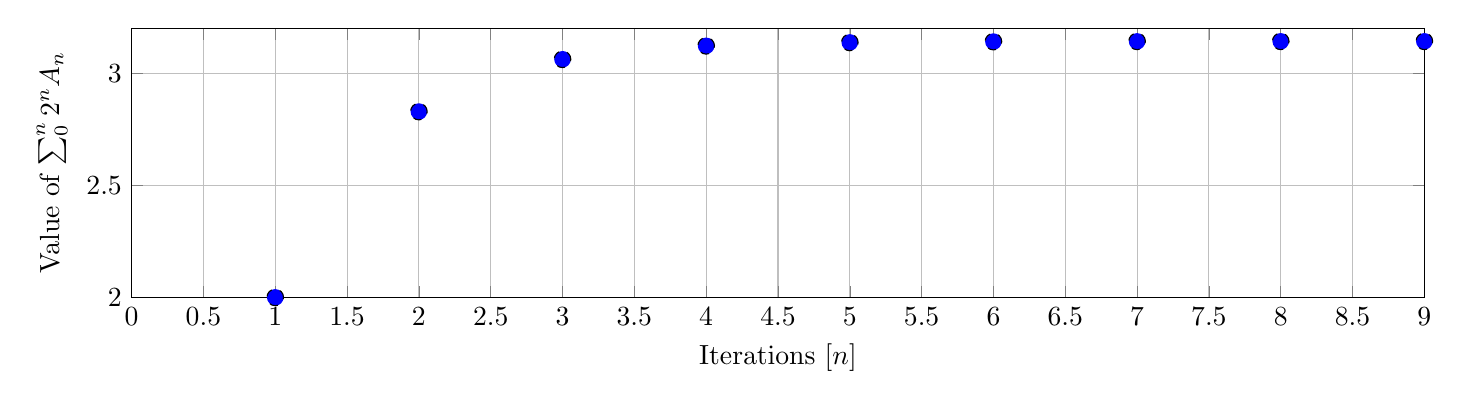
\begin{tikzpicture}

\begin{axis}[
xlabel={Iterations $[n]$},
ylabel={Value of $\sum_{0}^n2^nA_n$ },
xmin=0, xmax=9,
ymin=2, ymax=3.2,
axis on top,
width=18cm,
height=5cm,
xmajorgrids,
ymajorgrids
]
\addplot [blue, mark=*, mark size=3, mark options={dashed,draw=black}, only marks]
table {%
1 2
2 2.82842712474619
3 3.06146745892072
4 3.12144515225805
5 3.13654849054594
6 3.14033115695475
7 3.14127725093277
8 3.1415138011443
9 3.14157294036709
10 3.14158772527716
};
\end{axis}

\end{tikzpicture}
}
	\caption{Plot of values of series as a function of $n$}
	\label{fig:PISeriesPlot}
\end{figure}
As in Figure.\ref{fig:PISeriesPlot} we see that the series converges rapidly to the actual value of $\pi$. In just 4 iterations we get the value with error of only $0.001\%$.
\section{Discussion}
Value of $\pi$ thus can be calculated with the beautiful series without much hassle, the geometric nature of its derivation can clearly be understood by high school level students without much difficulty.  We hope this paper helps remove the common confusion among the beginners about what actually $\pi$ is -- a number whose value is between $3$ and $4$ in real line, precisely $3.141592653589$ for 14 digit precision as we have calculated with the series proposed in this paper. The number $\pi$ in essentially like any  other number in real number system, the only difference being the location of it in real line. 

\section{Conclusion}
We have constructed one series that is very intuitively easy to get to and converges very fast to the value of $\pi$. We have calculated the numerical value of the series which is $3.14159...$ \cite{fat}.

\section*{References}
\begin{thebibliography}{99}
	\bibitem{fat}
		H. Madhav and G. Prakash, The Delta Finders. The Delta Research Press (2016)
\end{thebibliography}
\end{document}
